\documentclass[11pt,letterpaper]{article}
\usepackage[T1]{fontenc}
\usepackage{lmodern}
\usepackage{graphicx}
\graphicspath{{./}{../}}
\providecommand{\pandocbounded}[1]{#1}
\usepackage{amsmath,amssymb,mathtools}
\usepackage[margin=1in,top=.85in,bottom=.85in]{geometry}
\usepackage{microtype}
\usepackage{enumitem}
\usepackage{titlesec}
\usepackage{needspace}
\usepackage[hidelinks]{hyperref}
\setlength{\parindent}{0pt}
\setlength{\parskip}{4.5pt plus 1pt minus 1pt}
\setlist{nosep,leftmargin=1.6em,topsep=4pt}
\setlength{\emergencystretch}{1.5em}
\allowdisplaybreaks[1]
\raggedbottom
\widowpenalty=10000
\clubpenalty=10000
\titleformat{\section}{\Large\bfseries}{}{0pt}{}
\titleformat{\subsubsection}{\normalsize\bfseries}{}{0pt}{}
\titleformat{\subsection}{\large\bfseries}{}{0pt}{}
\titlespacing*{\section}{0pt}{14pt}{8pt}
\titlespacing*{\subsubsection}{0pt}{9pt}{4pt}
\titlespacing*{\subsection}{0pt}{12pt}{6pt}
\newcommand{\tightlist}{\setlength{\itemsep}{0pt}\setlength{\parskip}{0pt}}
\hypersetup{pdftitle={Honours Linear Algebra - Week
1},pdfsubject={Honours Linear Algebra: 7 and 9 September 2026}}
\begin{document}
\begin{center}
{\LARGE Honours Linear Algebra - Week 1\par}
\vspace{5pt}
{\large 7 and 9 September 2026\par}
\end{center}
\vspace{4pt}
\Needspace{7\baselineskip}
\subsection{7 Sept.~/ Linear equations}\label{sept.-linear-equations}

\(A=(a_{ij})\in M_{m\times n}(\mathbb R)\): \(m\) rows, \(n\) columns.
Column vectors throughout. \[
\sum_{j=1}^n a_{ij}x_j=b_i\quad\longleftrightarrow\quad Ax=b,
\qquad[A\mid b]\in M_{m\times(n+1)}.
\] \textbf{Notation.} \[
\begin{aligned}
(A^T)_{ij}&=a_{ji},\quad A^T\in M_{n\times m},& I_n&=(\delta_{ij}),\\
(A+B)_{ij}&=a_{ij}+b_{ij},&(cA)_{ij}&=ca_{ij}.
\end{aligned}
\] Upper triangular: \(a_{ij}=0\) for \(i>j\); lower: \(i<j\); diagonal:
\(i\ne j\).

\textbf{Row operations.} \[
R_i\leftrightarrow R_j,\qquad R_i\leftarrow cR_i\ (c\ne0),\qquad
R_i\leftarrow R_i+cR_j\ (i\ne j).
\] All reversible \(\Rightarrow\) same solutions. Operate on the
right-hand side too.

\textbf{REF.} Zero rows last; leading \(1\)'s move right down the rows.
RREF: pivot columns zero elsewhere. This lecture takes pivots to be
\(1\).

\textbf{Solving.} Eliminate \(\to\) back substitute. For \(n\) variables
and \(r\) coefficient pivots: \[
\begin{array}{c|c}
[0\ \cdots\ 0\mid1]\text{ occurs}&\text{no solution}\\
\text{consistent},\ r=n&\text{unique}\\
\text{consistent},\ r<n&n-r\text{ free variables}
\end{array}
\]

\textbf{Ex.} Nonzero rows of the echelon system: \[
\begin{aligned}
x_1-x_2+4x_3+5x_4+4x_5&=0,\\
x_3+2x_4+6x_5&=1,\qquad x_5=3.
\end{aligned}
\] \(x_2=s\), \(x_4=t\) \(\Rightarrow x_3=-17-2t\), \(x_1=56+s+3t\). \[
x=\begin{pmatrix}56\\0\\-17\\0\\3\end{pmatrix}
+s\begin{pmatrix}1\\1\\0\\0\\0\end{pmatrix}
+t\begin{pmatrix}3\\0\\-2\\1\\0\end{pmatrix},\qquad s,t\in\mathbb R.
\] \textbf{Ex.} \(3x_1-9x_2=4\), \(-2x_1+6x_2=h\)
\(\Rightarrow 0=h+8/3\). Consistent iff \(h=-8/3\); then
\((x_1,x_2)=(4/3+3t,t)\).

\Needspace{4\baselineskip}
\textbf{Theorem.} Homogeneous, \(n>m\) \(\Rightarrow\) nonzero
solutions: \[
x=0\text{ solves it},\qquad n-r\ge n-m>0.
\] At least one free variable. Square RREF with \(n\) pivots \(=I_n\).

\newpage

\Needspace{7\baselineskip}
\subsection{9 Sept.~(I) / Inverse and LU}\label{sept.-i-inverse-and-lu}

\((AB)_{ij}=\sum_k a_{ik}b_{kj}\);
\((m\times n)(n\times p)\to m\times p\).

\textbf{Inverse.} \(AA^{-1}=A^{-1}A=I\); square \(A\) only. \[
A\text{ invertible}\iff Ax=b\text{ has exactly one solution for every }b.
\] Row-reduce \([A\mid I]\to[Q\mid E]\): \(Q=I\Rightarrow A^{-1}=E\);
otherwise no inverse.

Why: \(E=E_k\cdots E_1\) (elementary matrices), \(EA=I\). Each \(E_i\)
invertible \(\Rightarrow A=E^{-1}\Rightarrow AE=I\) too. \[
\begin{aligned}
(AB)^{-1}&=B^{-1}A^{-1},&(A^T)^{-1}&=(A^{-1})^T,\\
(B^{-1}A^{-1})(AB)&=I,&(A^{-1})^TA^T&=(AA^{-1})^T=I.
\end{aligned}
\] Other product orders similarly. Inverses reverse order.

\Needspace{4\baselineskip}
\textbf{Theorem.} Triangular + nonzero diagonal \(\Rightarrow\) inverse
triangular of the same type.

Upper case: solve \(Ax=e_j\) backwards. \(i>j\Rightarrow x_i=0\);
division only by \(a_{ii}\ne0\). These \(x\)'s form \(A^{-1}\).

\textbf{LU.} Elimination without row swaps: \[
E_k\cdots E_1A=U
\quad\Rightarrow\quad
A=LU,\quad L=E_1^{-1}\cdots E_k^{-1}.
\] \(L\): unit lower triangular; elimination multipliers below the
diagonal.

\textbf{Ex.} Opening matrix from \emph{The Nine Chapters}: \[
A=\begin{pmatrix}3&2&1\\2&3&1\\1&2&3\end{pmatrix},\qquad
\begin{aligned}
R_2&\leftarrow R_2-\tfrac23R_1,\\
R_3&\leftarrow R_3-\tfrac13R_1,\\
R_3&\leftarrow R_3-\tfrac45R_2.
\end{aligned}
\] \[
A=\underbrace{\begin{pmatrix}1&0&0\\2/3&1&0\\1/3&4/5&1\end{pmatrix}}_L
\underbrace{\begin{pmatrix}3&2&1\\0&5/3&1/3\\0&0&12/5\end{pmatrix}}_U.
\] \(Ax=b\): first \(Ld=b\) (forwards), then \(Ux=d\) (backwards). \[
b=\begin{pmatrix}39\\34\\26\end{pmatrix}
\Rightarrow d=\begin{pmatrix}39\\8\\33/5\end{pmatrix}
\Rightarrow x=\begin{pmatrix}37/4\\17/4\\11/4\end{pmatrix}.
\] With swaps: \(PA=LU\), so \(Ld=Pb\), \(Ux=d\). Slides' \(A=PLU\) uses
the inverse permutation.

Factor once \(O(n^3)\); each new \(b\): \(O(n^2)\). Reuse \(L,U\) rather
than form \(A^{-1}\).

\newpage

\Needspace{7\baselineskip}
\subsection{9 Sept.~(II) / Fields; vector
spaces}\label{sept.-ii-fields-vector-spaces}

\textbf{Def.1.1.} Field \(K\): \((K,+)\), \((K\setminus\{0\},\cdot)\)
abelian groups + distributivity; \(0\ne1\).

Examples: \(\mathbb Q,\mathbb R,\mathbb C\), \(\mathbb Q(\sqrt2)\),
\(\mathbb R(t)\), \(\mathbb F_p\) (\(p\) prime).
\(\mathbb Z/6\mathbb Z\) fails: \(2\cdot3=0\).

\textbf{Def.1.4.} Vector space over \(K\): addition \(V\times V\to V\),
scalar multiplication \(K\times V\to V\); for \(u,v,w\in V\),
\(c,d\in K\), \[
\begin{aligned}
u+v&=v+u,&(u+v)+w&=u+(v+w),\\
u+0&=u,&u+(-u)&=0,\\
(cd)u&=c(du),&1u&=u,\\
c(u+v)&=cu+cv,&(c+d)u&=cu+du.
\end{aligned}
\] \(0\in V\) and negatives must exist. Scalars \(\in K\); vectors
\(\in V\).

\textbf{Prop.1.5--7.} Unique zero, unique negative; cancellation;
\(cu=0\iff c=0\) or \(u=0\). \[
\begin{aligned}
0'&=0'+0=0,\\
u',u''\text{ negatives of }u:\quad
u'&=u'+(u+u'')=(u'+u)+u''=u'',\\
0u=(0+0)u=0u+0u&\Rightarrow0u=0,\\
c0=c(0+0)=c0+c0&\Rightarrow c0=0,\\
cu=0,\ c\ne0&\Rightarrow u=c^{-1}(cu)=0.
\end{aligned}
\] Cancellation: add \(-u\). Also
\(u+(-1)u=(1-1)u=0\Rightarrow(-1)u=-u\).

\Needspace{4\baselineskip}
\textbf{Examples.} \(\{0\}\), \(K^n\), \(M_{m\times n}(K)\), \(K[t]\).
Over \(\mathbb R\): \(C^0(\mathbb R)\); \(\{f:f''+f=0\}\), since \[
(af+bg)''+(af+bg)=a(f''+f)+b(g''+g)=0.
\] \(\mathbb C\) over \(\mathbb R\): yes. \(\mathbb R\) over
\(\mathbb C\): no, \(i\cdot1\notin\mathbb R\).

\textbf{Non-examples (usual operations).}

\begin{itemize}
\tightlist
\item
  \(x,y\ge0\): multiplying \((1,0)\) by \(-1\) leaves the set.
\item
  Invertible matrices; degree exactly \(n\); \(f(0)=1\): zero missing.
\item
  A line not through \(0\): same obstruction.
\end{itemize}

\newpage

\Needspace{7\baselineskip}
\subsection{Subspaces; span}\label{subspaces-span}

\begin{center}
\begin{minipage}{\linewidth}
\centering
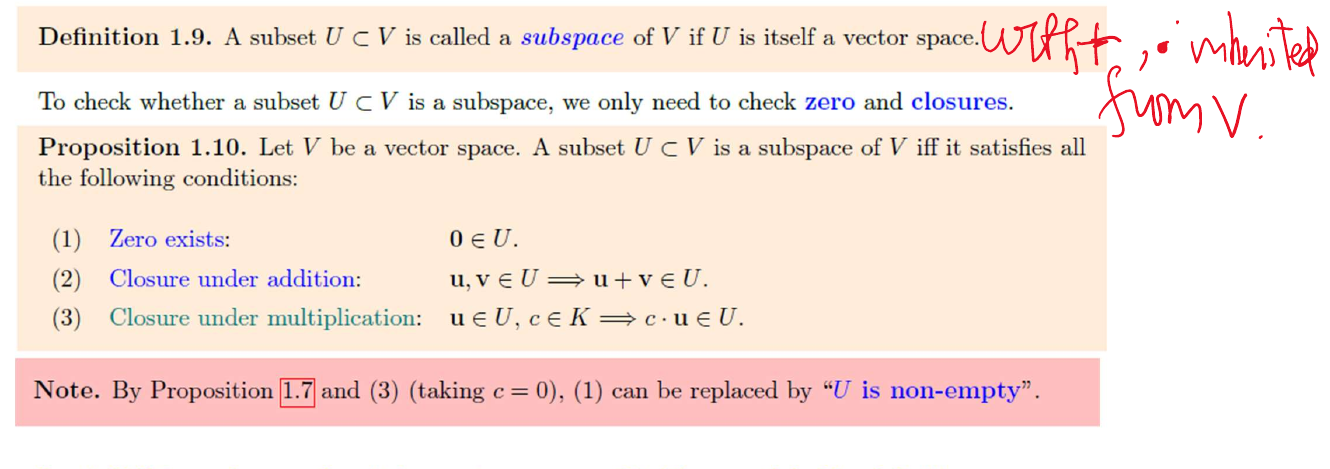
\includegraphics[width=0.9\linewidth,height=\textheight,keepaspectratio]{images/subspace-annotation.png}\par
{\small \emph{9 Sept., vector spaces, p.13.}\par}
\end{minipage}
\end{center}

\textbf{Test.} \(U\ne\varnothing\) and \(au+bv\in U\) for all
\(u,v\in U\), \(a,b\in K\). Identities inherited from \(V\);
\(-u=(-1)u\in U\).

Examples: \(x+y+z=0\) in \(\mathbb R^3\); \(K_n[t]\) (degree \(\le n\),
including \(0\)); \(\{f:f(0)=0\}\). \(\mathbb R^2\) itself is not a
subset of \(\mathbb R^3\); \(\{(x,y,0)^T\}\) is.

\textbf{Null space.} \(A\in M_{m\times n}(K)\): \[
\operatorname{Nul}(A)=\{x\in K^n:Ax=0\}\le K^n,
\qquad A(au+bv)=aAu+bAv=0.
\] \textbf{Def.1.11.}
\(\operatorname{Span}(S)=\{\text{finite linear combinations of vectors in }S\}\);
\(\operatorname{Span}(\varnothing)=\{0\}\).

\textbf{Thm.1.12.} \(\operatorname{Span}(S)\) is a subspace, the
smallest one containing \(S\). In particular
\(\operatorname{Span}(U)=U\) for a subspace \(U\).

Proof: add/scale combinations; still finite combinations. Any subspace
containing \(S\) contains all of them. \[
u_i=\sum_j a_{ij}v_j\quad\Rightarrow\quad
\sum_i c_i u_i=\sum_j\left(\sum_i c_i a_{ij}\right)v_j.
\] \textbf{Ex.1.27.} \[
\begin{pmatrix}a-3b\\b-a\\a\\b\end{pmatrix}
=a\begin{pmatrix}1\\-1\\1\\0\end{pmatrix}
+b\begin{pmatrix}-3\\1\\0\\1\end{pmatrix}.
\] \(a,b\in\mathbb R\) arbitrary
\(\Rightarrow U=\operatorname{Span}\{(1,-1,1,0)^T,(-3,1,0,1)^T\}\le\mathbb R^4\).

\textbf{Back to equations.} If \(Ax_p=b\), \[
Ax=b\iff A(x-x_p)=0
\iff x\in x_p+\operatorname{Nul}(A).
\] Homogeneous: subspace. Inhomogeneous: translate;
\(b\ne0\Rightarrow0\) not a solution.
\end{document}
